\documentclass[a4paper,11pt]{article}
\input{/home/tof/Documents/Cozy/latex-include/preambule_doc.tex}
\input{/home/tof/Documents/Cozy/latex-include/preambule_commun.tex}
\newcommand{\showprof}{show them}  % comment this line if you don't want to see todo environment
\setlength{\fboxrule}{0.8pt}
\fancyhead[L]{\fbox{\Large{\textbf{Tris 02}}}}
\fancyhead[C]{\textbf{Exercices tris - correction}}
\newdate{madate}{10}{09}{2020}
%\fancyhead[R]{\displaydate{madate}} %\today
%\fancyhead[R]{Seconde - SNT}
\fancyhead[R]{Première - NSI}
%\fancyhead[R]{Terminale - NSI}
\fancyfoot[L]{\vspace{1mm}Christophe Viroulaud}
\AtEndDocument{\label{lastpage}}
\fancyfoot[C]{\textbf{Page \thepage/\pageref{lastpage}}}
\fancyfoot[R]{\includegraphics[width=2cm,align=t]{/home/tof/Documents/Cozy/latex-include/cc.png}}
\usepackage{tikz}

\begin{document}
\begin{exo}
$$\dfrac{6,8×1000000^2}{16000^2}=26560s = 7h23min$$
\end{exo}
\begin{exo}
    \begin{center}
        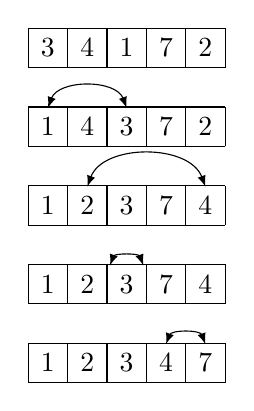
\begin{tikzpicture}[scale=0.5]
            \draw (0,0) grid (5,1);
            \node at(0.5,0.5) {3};
            \node at(1.5,0.5) {4};
            \node at(2.5,0.5) {1};
            \node at(3.5,0.5) {7};
            \node at(4.5,0.5) {2};

            
            \draw (0,-2) grid (5,-1);
            \node (1) at(0.5,-1.5) {1};
            \node at(1.5,-1.5) {4};
            \node (2)at(2.5,-1.5) {3};
            \node at(3.5,-1.5) {7};
            \node at(4.5,-1.5) {2};
            \draw[<->,>=latex] (1.north)to[bend left=70](2.north);

            \draw (0,-4) grid (5,-3);
            \node at(0.5,-3.5) {1};
            \node (3)at(1.5,-3.5) {2};
            \node at(2.5,-3.5) {3};
            \node at(3.5,-3.5) {7};
            \node (4)at(4.5,-3.5) {4};
            \draw[<->,>=latex] (3.north)to[bend left=70](4.north);

            \draw (0,-6) grid (5,-5);
            \node at(0.5,-5.5) {1};
            \node at(1.5,-5.5) {2};
            \node (5)at(2.5,-5.5) {3};
            \node at(3.5,-5.5) {7};
            \node at(4.5,-5.5) {4};
            \draw[<->,>=latex] (5.north west)to[bend left=70](5.north east);
    
            \draw (0,-8) grid (5,-7);
            \node at(0.5,-7.5) {1};
            \node at(1.5,-7.5) {2};
            \node at(2.5,-7.5) {3};
            \node (7)at(3.5,-7.5) {4};
            \node (8)at(4.5,-7.5) {7};
            \draw[<->,>=latex] (7.north)to[bend left=70](8.north);
        \end{tikzpicture}
        \captionof{code}{Tri par sélection}
        \end{center}

        \begin{center}
            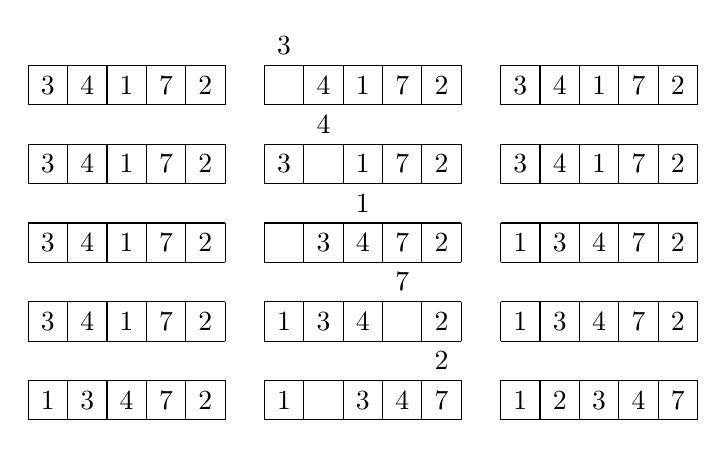
\begin{tikzpicture}[scale=0.5]
                \draw (0,0) grid (5,1);
                \node at(0.5,0.5) {3};
                \node at(1.5,0.5) {4};
                \node at(2.5,0.5) {1};
                \node at(3.5,0.5) {7};
                \node at(4.5,0.5) {2};

                \draw (6,0) grid (11,1);
                \node at(6.5,1.5) {3};
                \node at(7.5,0.5) {4};
                \node at(8.5,0.5) {1};
                \node at(9.5,0.5) {7};
                \node at(10.5,0.5) {2};

                \draw (12,0) grid (17,1);
                \node at(12.5,0.5) {3};
                \node at(13.5,0.5) {4};
                \node at(14.5,0.5) {1};
                \node at(15.5,0.5) {7};
                \node at(16.5,0.5) {2};
                %---
                \draw (0,-2) grid (5,-1);
                \node at(0.5,-1.5) {3};
                \node at(1.5,-1.5) {4};
                \node at(2.5,-1.5) {1};
                \node at(3.5,-1.5) {7};
                \node at(4.5,-1.5) {2};

                \draw (6,-2) grid (11,-1);
                \node at(6.5,-1.5) {3};
                \node at(7.5,-0.5) {4};
                \node at(8.5,-1.5) {1};
                \node at(9.5,-1.5) {7};
                \node at(10.5,-1.5) {2};

                \draw (12,-2) grid (17,-1);
                \node at(12.5,-1.5) {3};
                \node at(13.5,-1.5) {4};
                \node at(14.5,-1.5) {1};
                \node at(15.5,-1.5) {7};
                \node at(16.5,-1.5) {2};
                %---
                \draw (0,-4) grid (5,-3);
                \node at(0.5,-3.5) {3};
                \node at(1.5,-3.5) {4};
                \node at(2.5,-3.5) {1};
                \node at(3.5,-3.5) {7};
                \node at(4.5,-3.5) {2};

                \draw (6,-4) grid (11,-3);
                \node at(7.5,-3.5) {3};
                \node at(8.5,-3.5) {4};
                \node at(8.5,-2.5) {1};
                \node at(9.5,-3.5) {7};
                \node at(10.5,-3.5) {2};

                \draw (12,-4) grid (17,-3);
                \node at(13.5,-3.5) {3};
                \node at(14.5,-3.5) {4};
                \node at(12.5,-3.5) {1};
                \node at(15.5,-3.5) {7};
                \node at(16.5,-3.5) {2};
                %---
                \draw (0,-6) grid (5,-5);
                \node at(0.5,-5.5) {3};
                \node at(1.5,-5.5) {4};
                \node at(2.5,-5.5) {1};
                \node at(3.5,-5.5) {7};
                \node at(4.5,-5.5) {2};

                \draw (6,-6) grid (11,-5);
                \node at(7.5,-5.5) {3};
                \node at(8.5,-5.5) {4};
                \node at(6.5,-5.5) {1};
                \node at(9.5,-4.5) {7};
                \node at(10.5,-5.5) {2};

                \draw (12,-6) grid (17,-5);
                \node at(13.5,-5.5) {3};
                \node at(14.5,-5.5) {4};
                \node at(12.5,-5.5) {1};
                \node at(15.5,-5.5) {7};
                \node at(16.5,-5.5) {2};
                %---
                \draw (0,-8) grid (5,-7);
                \node at(0.5,-7.5) {1};
                \node at(1.5,-7.5) {3};
                \node at(2.5,-7.5) {4};
                \node at(3.5,-7.5) {7};
                \node at(4.5,-7.5) {2};

                \draw (6,-8) grid (11,-7);
                \node at(6.5,-7.5) {1};
                \node at(8.5,-7.5) {3};
                \node at(9.5,-7.5) {4};
                \node at(10.5,-7.5) {7};
                \node at(10.5,-6.5) {2};

                \draw (12,-8) grid (17,-7);
                \node at(12.5,-7.5) {1};
                \node at(13.5,-7.5) {2};
                \node at(14.5,-7.5) {3};
                \node at(15.5,-7.5) {4};
                \node at(16.5,-7.5) {7};
                %---
            \end{tikzpicture}
            \captionof{code}{Tri par insertion}
            \end{center}
\end{exo}
\begin{exo}
Il faut copier ou importer la fonction \textbf{\texttt{tri\_selection}}.
\lstinputlisting[firstline=28 ,lastline=39 ]{"scripts/comparer.py"}
\end{exo}
\begin{exo}
\lstinputlisting[firstline=12 ,lastline=31]{"scripts/tri-insertion.py"}
\end{exo}
\begin{exo}
\lstinputlisting[firstline=12 ,lastline=25 ]{"scripts/tri-stable.py"}
Le tri par insertion est un tri stable. Ce n'est pas le cas du tri par sélection.
\end{exo}
\begin{exo}
\lstinputlisting[firstline=28 ,lastline=49 ]{"scripts/compter.py"}
\end{exo}
\begin{exo}
\lstinputlisting[firstline=12 ,lastline=28 ]{"scripts/tri-bulles.py"}
\end{exo}
\end{document}